\section{Preliminaries}

Following \cite{Zheng2017}, the framework for solving the RE task consists of two modules:
{\em RE tagging module} and {\em triple construction algorithm}.

% In this paper, following the system of \citet{Zheng2017}, there are two module in
% the whole system, RE tagging module and triple construction algorithm. First
% {\em label} each word in the sentence with a RE tag, and
% second {\em reconstruct} the relation triples from the tag sequence.

\figref{fig:intro} shows a an example of the tagging scheme. For example, in
``LE-1-B'' (for Tim),
``LE'' is the abbreviation of ``LeaderOf'', ``1'' means both ``Tim'' is  $e_1$
of ``LeaderOf'' relation, ``B'' means ``Tim'' is the beginning of this entity.


RNN can be used to decode the RE tags. \figref{fig:model} is the framework
for this problem. The the input is word sequence of a sentence. After the word
embedding layer, a BiLSTM is used to extract low level features. The a forward
LSTM and a softmax layer is used to decode the tag sequence. Finally, the
relation triple construction algorithm will reconstruct mentioned tirples from
predicted tag sequence.


\begin{figure}[h!]
\centering
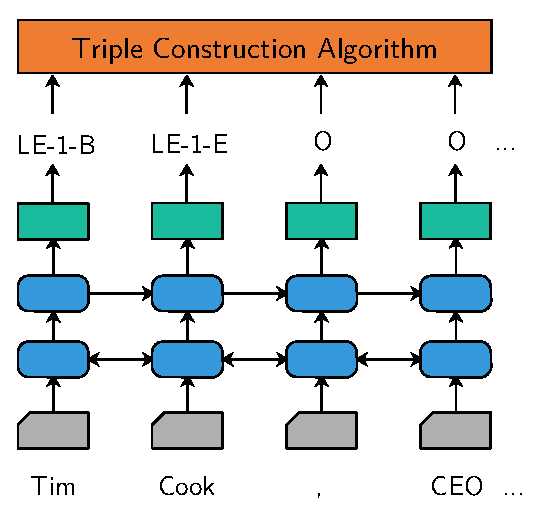
\includegraphics[width=4.5cm]{pictures/model.eps}
\caption{Sequential tagging framework for relation extraction \cite{Zheng2017}. \label{fig:model}}
\end{figure}



